\section{Methods}
\label{app:methods}

\subsection{Two-layer model: architecture, data and optimization}
The two-layer model is an attention-only causal transformer with width
256, eight heads per layer, context length 128, pre-layer normalization, and
689,664 trainable parameters. Learned position vectors enter the query and key
streams but not the value stream. Training minimizes next-byte cross-entropy with
batch size 64 and AdamW (learning rate $10^{-3}$, betas $(0.9,0.98)$, weight decay
0.1, 200 warm-up updates). Every condition begins with the same 2,000-update
warm-up on unmodified text for its seed.

All corpora derive from one 100\,MB order-2 Eulerian shuffle of enwik8, which
preserves byte-bigram counts but destroys longer-range structure. The base corpus
is this shuffle. The short-repeat corpus copies 16-byte spans forward by a
uniformly sampled distance in 17--31 at 400,000 seeded sites. The long-repeat
(target) corpus copies 32-byte spans forward by a distance in 40--88 at 170,000
sites. Training crops start below byte 90M; held-out evaluations start at byte
95M. Each corpus has its own deterministic crop-position generator, so moving a
block of training in time changes when a batch is seen but not which batches are
seen or in what order. Replay rewinds only the target generator. Every
result record stores source counts, generator state, corpus hashes and a digest
of all crop positions, and the scorers reject any mismatch.

\emph{Copy gain} (\texttt{uptake} in the implementation code) is
$\mathrm{CE}_{\text{base}}(\theta;M)-\mathrm{CE}_{\text{target}}(\theta;M)$, where both
cross-entropies are computed at the positions $M$ inside pasted spans, on paired
crops of the unmodified and target corpora. The key probe presents a four-byte key
twice and asks for the byte that followed its first occurrence, at distances 24,
64 and 96 (256 examples each, drawn from the 96 most frequent bytes and generated
independently of the training data). Unless stated otherwise, we evaluate every
500 updates, and endpoint values average the final five evaluations.

\paragraph{Formation rule and schedules.}
After the shared warm-up, the \emph{prerequisite-first} schedule trains on short
repeats until two consecutive distance-24 probe evaluations are at least 0.70, no
earlier than update 10,000 and with a 120,000-update cap, then trains on 90,000
target batches. The \emph{target-first} schedule consumes the same 90,000 target
batches first, then exactly as many short-repeat batches as its paired
prerequisite-first run used (Table~\ref{tab:g1core}).

\begin{table}[!htbp]
\centering\small
\caption{Order comparison with fixed data in the two-layer model. Copy gain is the
maximum in the first 10,000 target updates; the endpoint averages the last five
evaluations. \emph{Data match} requires equal target batch counts and position
digests within each seed.}
\label{tab:g1core}
\begin{tabular}{lrrrrrl}\toprule
 & & \multicolumn{2}{c}{prerequisite first} & \multicolumn{2}{c}{target first} & \\
\cmidrule(lr){3-4}\cmidrule(lr){5-6}
seed & formation update & copy gain $\le$10k & end $d{=}64$ & copy gain $\le$10k & end $d{=}64$ & data match\\\midrule
531 & 59,500 & 2.57 & 0.52 & 0.00 & 0.01 & yes \\
532 & 40,000 & 2.40 & 0.52 & 0.03 & 0.00 & yes \\
533 & 84,000 & 2.58 & 0.61 & -0.03 & 0.01 & yes \\
\bottomrule\end{tabular}
\end{table}

\subsection{Two-layer model: circuit identification and interventions}
\label{app:interventions}
In each model in which the prerequisite has formed, we zero each head's output in
turn. The circuit is every head whose individual removal lowers distance-24
accuracy by at least 45\% of its intact value, capped at four per layer. Controls are equally many
heads with at most a 15\% drop, matched by layer where possible (one control in
seed 532 comes from the other layer). We set this rule after seeing the first
two identification tables and applied it unchanged to the third seed and to all
later seeds. Table~\ref{tab:circuits} gives the selected heads and manipulation
checks.

\emph{Reset} redraws a head's query, key, value, and output weights from the
model's original initialization distribution with a recorded seed; the model then
receives a fresh AdamW optimizer and the first 90,000 batches of the same target
stream. The conditions are \emph{no edit}; \emph{control reset}; \emph{circuit
reset} (all selected heads); \emph{age-matched control} (the warm-up state after an
equal number of additional base-corpus updates); \emph{previous-token reset} (the
largest-effect first-layer head only); \emph{induction-head reset} (every selected
second-layer head); and \emph{heads frozen} (the weights of the six selected heads
are fixed, but gradients still pass through them).

\begin{table}[!htbp]
\centering\small
\caption{Per-seed circuit identification. Heads are layer.head. The
joint-ablation columns report distance-24 accuracy after zeroing the circuit or the
controls.}
\label{tab:circuits}
\resizebox{\linewidth}{!}{%
\begin{tabular}{lrlrlr}\toprule
seed & intact $d{=}24$ & circuit heads & joint ablation & control heads & joint ablation\\\midrule
531 & 0.73 & 1.2, 1.7, 1.0, 2.7, 2.3, 2.6 & 0.012 & 1.1, 1.4, 1.6, 2.5, 2.2, 2.0 & 0.72 \\
532 & 0.72 & 1.3, 1.2, 1.7, 1.5, 2.6, 2.0 & 0.004 & 1.6, 1.4, 1.0, 2.1, 2.3, 2.2 & 0.81 \\
533 & 0.73 & 1.5, 1.6, 1.0, 2.6, 2.5, 2.4 & 0.020 & 1.3, 1.7, 1.4, 2.0, 2.2, 2.3 & 0.82 \\
\bottomrule\end{tabular}}
\end{table}

\paragraph{Training-only suppression with exact restoration.}
Each model uses its previous-token head (the largest-effect first-layer head) and a
low-effect first-layer control head, chosen from the identification records by the
smallest absolute change in base-text loss. We freeze the query, key and value rows
and output columns of both heads, the token embeddings, the positions and the first
normalization. The two heads receive the same first-layer inputs, so this fixes
their complete input path (164,352 parameters). Everything else trains.

The unsuppressed, control-suppressed and suppressed conditions receive the first
1,000 target batches. A fourth condition suppresses the previous-token head while
training on unmodified text at the same crop positions. Every evaluation enables
both heads.

To supply the head's output, we use the same models and freezing. We suppress the
previous-token head's own output in every training forward pass and add one of
three signals to the first-layer attention output: the head's intact contribution,
computed by a frozen copy of the starting model on the same tokens; the control
head's contribution; or nothing. Supplied activations are detached. We do not rescale
the wrong-head supply, so activation norms are not matched. Every evaluation
disables both suppression and supply. The correct supply reproduces the
unsuppressed forward pass to within $2.1\times10^{-5}$ in the logits on fixed audit
sequences.

\subsection{Pretrained models}
\label{app:pythiamethods}
\paragraph{Batches and optimization.}
One optimizer update uses 18 sequences of length 128, in micro-batches of six,
with AdamW (betas $(0.9,0.95)$, weight decay 0.01, gradient-norm clipping at 1) in
FP32. The original 160M studies use learning rate $10^{-4}$ and 500 updates. The
scaling studies use $3\times10^{-5}$. We chose this rate by a search over
$\{3\times10^{-5},10^{-5},3\times10^{-6}\}$ that used only unsuppressed and control
runs on separate development streams; it is the first rate in the search at which
every control learned. In the order and replay study, the induction-forming batch
contains six natural-text windows with six copied six-token spans, six random-token
sequences with six copied spans and six untouched natural windows (copy distances
24--64).

\paragraph{Target batches and probes.}
A target batch contains six mapped-copy sequences, six ordinary induction
sequences (random tokens with a four-token key repeated 24--64 tokens later) and
six natural-text windows. In mapped copy, the token after the first key is one of
32 reserved markers, three distractor markers make the source ambiguous, and the
correct continuation of the repeated key is the marker's image under a fixed random
involution. Accuracy is the full-vocabulary argmax at the query position.

Probes contain 256 held-out sequences, and natural-text loss uses 64 held-out
windows. Each target-stream seed determines both the data and the involution. The
scaling studies use a corrected version of the ordinary-induction training rows, in
which the token after the repeated key is the copied continuation; in the original
implementation it was random. The correction changes no qualitative outcome at 160M, 410M
or 1B (\appref{app:scaling}).

\paragraph{Head selection.}
On an ordinary induction probe (seed 1701), we record each head's attention from
the query (the last token of the repeated key) to the source (the token after the
key's first occurrence). Circuit sets are the top-$k$ heads for increasing $k$.
Controls take, in each layer of the circuit set, the lowest-attention head not
already chosen. We select the smallest $k$ for which, on two calibration probes,
suppressing the circuit leaves induction accuracy at most 0.02 (0.2 in the
original 160M study) with a drop of at least 0.3, while the controls retain at
least 0.5 with a drop of at most 0.15. A new 1,024-example probe verifies the
choice. Where the lowest-attention controls remove too much induction (1.4B, 6.9B
and 12B), we search for layer-matched controls among heads in the lower half of
attention scores. Table~\ref{tab:selection} lists the selections.

\paragraph{Key-dependence tests.}
The \emph{key-swap} test exchanges the true source's four-token key with the four
tokens before a different-valued distractor in the legal window. This keeps the
query, all marker identities and positions, and the multiset of tokens fixed, but
changes the correct answer, so no rule that uses only marker identities and
positions can answer both versions. Eligible pairs are determined without model
outcomes (typically 130--150 of 256 examples). The \emph{key-deletion} test
replaces the true key with unused tokens. The nearest-marker heuristic scores
60.2--60.5\%.

\section{What was fixed in advance}
\label{app:hygiene}
Head selections use only induction probes, never target outcomes, and we choose
learning rates on control and unsuppressed runs only. We wrote down the learning
criteria, training lengths and evaluation schedules before the corresponding target runs.
We report every planned model, seed and pretraining run, including failures. We
calibrated the head-selection threshold of the two-layer model on the first two
seeds and applied it unchanged thereafter.

In the two-layer model the replication unit is the initialization and data seed.
In Pythia it is the public pretraining run, and the two target streams within a run
are technical replicates.

Several analyses are post hoc, and we label them as such where they appear: the
timing analysis of delayed learning (\secref{sec:scaling}), the per-head attention
analyses (\appref{app:regrowth}) and the initial-score comparison in
\appref{app:resets}. We designed the adaptive-suppression, loss-matched-control,
longer-training and additional-seed experiments after the main scaling results
were known, but fixed their rules before their own outcomes. Interrupted runs
resume from saved model, optimizer and data-stream state, and we checked that the
overlapping evaluations match exactly.

The follow-up experiments added for this version have the following history. A
first key-triggered variant used plain target accuracy under the mask (threshold
0.10) as its score. That score sits near its noise floor from the start
(0.05--0.10 before any key-dependent learning), so it triggered on noise. We stopped
those runs at update 400--500 and replaced the score with the key-swap pass rate
before any key-triggered outcome was known; we do not report the stopped runs.

The first 2.8B launch ran out of GPU memory at update 0, and we restarted it from
scratch. We stopped the 160M loss-matched runs at update 600 to free memory and
reran them from scratch with identical settings; the rerun matches the stopped run
at every shared evaluation. We paused one independent 410M run (process suspended)
and resumed it without changing its state. We designed the adaptive procedures, the
13-head mask rule, the static and yoked controls, the loss-matched selection and the
160M dose runs after seeing that models with fixed masks eventually learn, but fixed
their rules before their own outcomes.

\section{Complete results for the two-layer model}
\label{app:controlled}

\begin{figure}[!htbp]
\centering
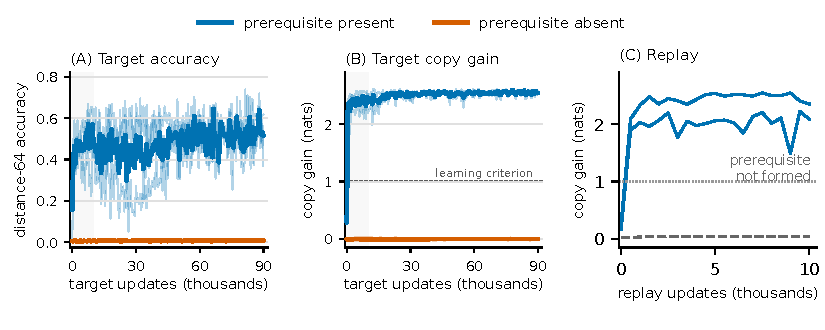
\includegraphics[width=\linewidth]{fig_orders.pdf}
\caption{\textbf{The same data teach only after the prerequisite forms}
(two-layer model). (A--B) Within each seed, both schedules receive the same
90,000 target batches in the same order, either after the induction circuit forms
(blue) or before it (orange). Thin lines are three seeds and thick lines are means;
the shaded region is the 10,000-update learning window. (C) Replay: the
model sees the target stream, then short repeats, then the identical target stream
again. The two models in which the circuit formed learn on replay; the model in
which it did not form (gray) does not.}
\label{fig:orders}
\end{figure}

\begin{table}[!htbp]
\centering\small
\caption{Outcomes of all circuit interventions in the three original models.
Start accuracy is measured immediately after the edit. \emph{First $\ge$1 nat} is
the first evaluation that crosses the criterion; \emph{none} means no crossing in
90,000 updates.}
\label{tab:c1core}
\resizebox{.94\linewidth}{!}{%
\begin{tabular}{llrrrrl}\toprule
seed & intervention & start $d{=}24$ & copy gain $\le$10k & first $\ge$1 nat & end $d{=}64$ & outcome\\\midrule
531 & No edit & 0.73 & 2.56 & 500 & 0.47 & learned \\
531 & Control reset & 0.70 & 2.53 & 500 & 0.61 & learned \\
531 & Circuit reset & 0.01 & 0.00 & none & 0.01 & not learned \\
531 & Age-matched control & 0.01 & 0.00 & none & 0.01 & not learned \\
531 & Previous-token reset & 0.01 & 0.00 & none & 0.01 & not learned \\
531 & Induction-head reset & 0.02 & 2.46 & 500 & 0.32 & learned \\
531 & Heads frozen & 0.73 & 2.50 & 500 & 0.60 & learned \\
532 & No edit & 0.72 & 2.40 & 500 & 0.50 & learned \\
532 & Control reset & 0.82 & 2.38 & 500 & 0.69 & learned \\
532 & Circuit reset & 0.01 & 0.02 & none & 0.00 & not learned \\
532 & Age-matched control & 0.01 & 0.02 & none & 0.00 & not learned \\
532 & Previous-token reset & 0.01 & 0.02 & none & 0.00 & not learned \\
532 & Induction-head reset & 0.03 & 2.39 & 500 & 0.59 & learned \\
532 & Heads frozen & 0.72 & 2.40 & 500 & 0.77 & learned \\
533 & No edit & 0.73 & 2.58 & 500 & 0.63 & learned \\
533 & Control reset & 0.76 & 2.59 & 500 & 0.63 & learned \\
533 & Circuit reset & 0.02 & -0.03 & none & 0.01 & not learned \\
533 & Age-matched control & 0.01 & -0.03 & none & 0.01 & not learned \\
533 & Previous-token reset & 0.02 & -0.02 & none & 0.01 & not learned \\
533 & Induction-head reset & 0.04 & 2.57 & 500 & 0.60 & learned \\
533 & Heads frozen & 0.73 & 2.56 & 500 & 0.62 & learned \\
\bottomrule\end{tabular}}
\end{table}

\begin{table}[!htbp]
\centering\small
\caption{Replay within one model. Copy gain columns are maxima over the full
first exposure and the first 10,000 replay updates. \emph{Exact} verifies that the
generator was rewound and that both presentations used the same 90,000 batches in
the same order.}
\label{tab:replay}
\begin{tabular}{llrrrrl}\toprule
seed & circuit formed & first exposure & replay $\le$10k & first $\ge$1 nat & replay end $d{=}64$ & exact\\\midrule
531 & yes & 0.00 & 2.22 & 500 & 0.55 & yes \\
532 & no (cap) & 0.03 & 0.05 & -- & 0.00 & yes \\
533 & yes & -0.02 & 2.55 & 500 & 0.75 & yes \\
\bottomrule\end{tabular}
\end{table}

\paragraph{Training-only suppression and replay afterwards.}
Table~\ref{tab:stable} reports every endpoint of the suppression experiment. After
the suppressed exposure, the suppressed and unmodified-text conditions receive
exact target replay with both heads enabled and fresh optimizers. No model learns
immediately when the suppressed head is re-enabled.

Replay afterwards gives mixed results. In seed 531 the model learns after
suppressed target exposure but not after unmodified-text exposure, which is
compatible with a latent benefit from the suppressed exposure. Seed 532 learns in
neither case, and seed 533 learns in both. Re-enabling a head therefore guarantees
neither that the heads reading its output remain compatible nor that replay
recovers within 1,000 updates.

\begin{table}[htbp]\centering\small
\caption{Training-only suppression and subsequent replay (copy gain in nats, both
heads enabled). Each phase lasts 1,000 updates. The last two columns start from the
suppressed-target and unmodified-text endpoints.}\label{tab:stable}
\begin{tabular}{lllllll}\toprule
seed & unsuppressed & control & suppressed & unmodified text & replay & text + target \\
\midrule
531 & 2.366 & 2.368 & -0.002 & -0.005 & 1.546 & 0.008 \\
532 & 2.295 & 2.292 & 0.022 & 0.021 & 0.032 & 0.028 \\
533 & 2.481 & 2.453 & -0.029 & -0.034 & 2.366 & 2.332 \\
\bottomrule\end{tabular}
\end{table}

\begin{table}[htbp]\centering\small
\caption{Supplying the head's output, evaluated with the intact head. Entries are copy gain
(nats) / distance-64 accuracy after 1,000 updates.}\label{tab:supply}
\begin{tabular}{llll}\toprule
seed & correct supply & no supply & wrong-head supply \\
\midrule
531 & 2.366 / 0.438 & -0.002 / 0.012 & -0.002 / 0.012 \\
532 & 2.295 / 0.336 & 0.022 / 0.004 & 0.022 / 0.004 \\
533 & 2.481 / 0.340 & -0.029 / 0.008 & -0.030 / 0.008 \\
\bottomrule\end{tabular}
\end{table}

\paragraph{Additional seeds.}
Five further seeds, trained from scratch under the same rules, replicate both the
suppression result and the result of supplying the head's output
(\appref{app:newseeds}).

\paragraph{Transfer and restricted plasticity.}
We transfer the six selected heads, together with the token embeddings, positions,
readout and all normalizations, from a model in which the prerequisite has formed
into its own earlier (warm-up) checkpoint. The transferred model learns the target
task; transferring six control heads with the same interface does not help
(Table~\ref{tab:transfer}). The transfer changes 52.5\% of parameters, and neither
the heads alone nor the heads with positions install the prerequisite. The result
therefore shows transfer of learned weights, not a minimal circuit transplant.

Holding the weights of the selected heads fixed still permits 1.86--2.36 nats of
copy gain by 500 updates, and training only those heads also yields copy gain. The
adaptation that follows the circuit therefore has no unique location.

\begin{table}[htbp]\centering\small
\caption{Transfer and restricted plasticity (copy gain in nats; the maximum
excludes update zero; endpoint accuracy averages the last five
evaluations).}\label{tab:transfer}
\begin{tabular}{lllll}\toprule
seed & intervention & initial & max $\le$10k & end $d{=}64$ \\
\midrule
531 & Circuit transfer & 0.142 & 2.533 & 0.594 \\
531 & Control transfer & -0.001 & -0.003 & 0.014 \\
531 & Only heads train & 0.259 & 2.503 & 0.105 \\
532 & Circuit transfer & 0.289 & 2.388 & 0.634 \\
532 & Control transfer & 0.017 & 0.024 & 0.003 \\
532 & Only heads train & 0.266 & 2.417 & 0.579 \\
533 & Circuit transfer & 0.390 & 2.526 & 0.524 \\
533 & Control transfer & -0.042 & -0.030 & 0.007 \\
533 & Only heads train & 0.337 & 2.534 & 0.478 \\
\bottomrule\end{tabular}
\end{table}

\section{Resetting the previous-token head or the induction heads}
\label{app:resets}

\begin{figure}[htbp]
\centering
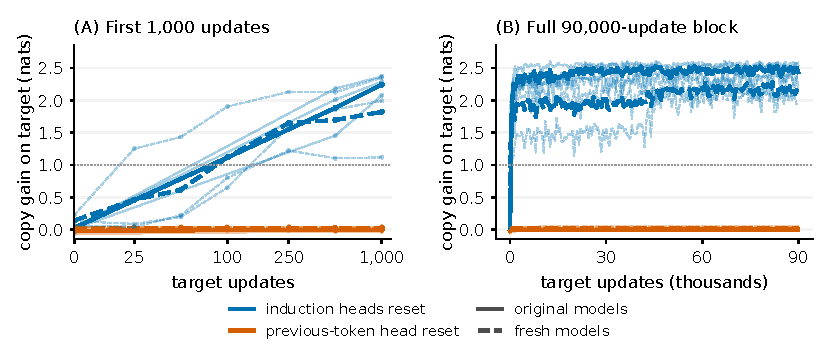
\includegraphics[width=\linewidth]{fig_hero.pdf}
\caption{\textbf{Resetting the previous-token head blocks learning; resetting the
induction heads does not.} All parameters train on the same target stream after
either the largest-effect first-layer (previous-token) head is reset (orange) or the
selected second-layer (induction) heads are reset (blue). (A) First 1,000 updates
(axis linear to 25 updates, logarithmic after). (B) The full 90,000 updates. Thin
lines are three original (solid) and three fresh (dashed) models; thick lines are
means.}
\label{fig:hero}
\end{figure}

Resetting the previous-token head changes 4.8\% of the parameters and changes
base-text loss by at most 0.01 nats relative to no edit. In the three original
models and three fresh models (seeds 1541--1543, run under the same pre-specified
rules), it blocks learning throughout 90,000 target updates. Resetting the selected
second-layer (induction) heads instead lets all six models learn within 500 updates
(\figref{fig:hero}). Control resets preserve learning.

Both resets reduce initial short-range accuracy to at most 0.036 in the original
models. In the fresh models, however, a pre-specified test of equal initial
impairment on the target failed (Table~\ref{tab:mfc_initial}): after the
induction-head reset the models start slightly better on the target (by 1--8
percentage points of distance-64 accuracy and 0.07--0.23 nats of loss). The
comparison therefore shows a difference in recovery between two specific lesions,
not between equally impaired models.

A second group of fresh models (seeds 2641--2643) resets \emph{all} eight second-layer heads
and the output readout. This broader lesion starts no better than the previous-token
reset on either target measure and does not recover within 10,000 updates
(Tables~\ref{tab:dominanceinitial}--\ref{tab:dominancerecovery}). Damage to the
second layer is thus not always easy to repair: within this budget the model
rebuilds the selected induction heads but not the whole second layer and readout.
In the same group the previous-token reset blocks learning in two models and allows
it (at update 3,000) in the third, which \appref{app:retained} explains.

\begin{table}[!htbp]
\centering\small
\caption{Pre-specified initial matching in the fresh reset models. P and S denote
the previous-token reset and the reset of the selected second-layer heads; correct
counts are out of 4,096 per condition. Intervals use a simultaneous 0.05 error
allocation. Matching requires the accuracy interval within $\pm2$ percentage points,
the loss interval within $\pm0.1$ nats and both accuracy upper bounds at most
0.05.}
\label{tab:mfc_initial}
\begin{tabular}{lrccrr}\toprule
 & correct & \multicolumn{2}{c}{P $-$ S interval} & floor & \\
\cmidrule(lr){3-4}
seed & P/S & accuracy (pp) & target CE (nats) & $\le .05$ & matched\\\midrule
1541 & 47/163 & [-4.21, -1.45] & [0.098, 0.121] & yes & no \\
1542 & 31/282 & [-7.67, -4.57] & [0.195, 0.233] & no & no \\
1543 & 40/99 & [-2.59, -0.28] & [0.069, 0.085] & yes & no \\
\bottomrule\end{tabular}
\end{table}

\begin{table}[!htbp]
\centering\small
\caption{Learning in the fresh models after the previous-token reset (P) or the
reset of the selected second-layer heads (S) over the full 90,000-update stream, and
with no edit or a control reset (I/C) over 10,000. \emph{S first} is the first
observed copy gain $\ge$1 nat; no P condition reaches it.}
\label{tab:mfc_recovery}
\begin{tabular}{lrrcrr}\toprule
seed & P max & S at 500 & S first & end $d{=}64$ P/S & end copy gain I/C\\\midrule
1541 & 0.043 & 1.856 & 250 & 0.008/0.605 & 2.154/2.158 \\
1542 & 0.054 & 2.125 & 25 & 0.012/0.516 & 2.054/2.085 \\
1543 & -0.008 & 1.101 & 250 & 0.004/0.613 & 1.936/1.931 \\
\bottomrule\end{tabular}
\end{table}

\begin{table}[!htbp]
\centering\small
\caption{Initial impairment in the broader-lesion group (P is the previous-token
reset; S resets all second-layer heads and the readout). Gaps are S minus P with
paired 95\% intervals.}
\label{tab:dominanceinitial}
\begin{tabular}{@{}lllll@{}}\toprule
seed & accuracy P/S & loss P/S & accuracy gap (pp) & loss gap (nats) \\
\midrule
2641 & 0.008/0.005 & 2.703/5.799 & [-0.659, 0.024] & [3.081, 3.112] \\
2642 & 0.010/0.004 & 2.704/5.726 & [-0.965, -0.256] & [3.007, 3.038] \\
2643 & 0.011/0.004 & 2.713/5.705 & [-1.093, -0.323] & [2.976, 3.007] \\
\bottomrule\end{tabular}
\end{table}

\begin{table}[!htbp]
\centering\small
\caption{Broader-lesion group over 10,000 target updates.}
\label{tab:dominancerecovery}
\begin{tabular}{@{}lllll@{}}\toprule
seed & intact first & first P/S & end copy gain P/S & end $d{=}64$ P/S \\
\midrule
2641 & 25 & none/none & 0.010/0.008 & 0.012/0.012 \\
2642 & 50 & 3000/none & 1.472/0.015 & 0.363/0.023 \\
2643 & 250 & none/none & -0.020/-0.020 & 0.008/0.008 \\
\bottomrule\end{tabular}
\end{table}

\section{Long training without the prerequisite}
\label{app:horizon}

\begin{figure}[htbp]
\centering
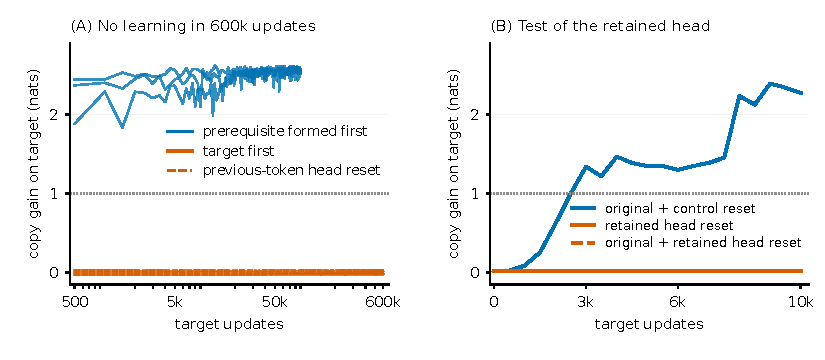
\includegraphics[width=\linewidth]{fig_mechanism.pdf}
\caption{\textbf{Persistent failure and the retained previous-token head.}
(A) Six continuations without the prerequisite (target first and previous-token
reset, three seeds each) stay below 0.03 nats through 600,000 updates; with the
prerequisite, the model learns within 500 updates (logarithmic axis). (B) In the
one model that learned after the previous-token reset, resetting its remaining
previous-token head blocks learning; an equally large control reset does not.}
\label{fig:mechanism}
\end{figure}

For each original seed, the target-first model repeats the warm-up and trains
continuously from target batch zero to 600,000. The previous-token-reset model
restores its archived 90,000-update model and optimizer state, verifies the
data-stream position and trains a further 510,000 updates. We evaluate every 500
updates. A memory fault at launch required restarting from the warm-up and the
archived endpoint, respectively; no outcome informed the restart, and we replace no
seed (Table~\ref{tab:longhorizon}). The 1,200-fold comparison uses learning by 500
updates when the prerequisite is present.

\begin{table}[!htbp]
\centering\small
\caption{Long continuations without the prerequisite. End values average the
last five evaluations.}
\label{tab:longhorizon}
\begin{tabular}{lllllll}\toprule
seed & condition & updates & max copy gain & first $\ge$1 nat & end copy gain & end $d{=}64$ \\
\midrule
531 & target first & 600,000 & 0.00 & none & -0.01 & 0.01 \\
531 & previous-token reset & 600,000 & 0.00 & none & 0.00 & 0.01 \\
532 & target first & 600,000 & 0.03 & none & 0.02 & 0.00 \\
532 & previous-token reset & 600,000 & 0.03 & none & 0.02 & 0.00 \\
533 & target first & 600,000 & -0.02 & none & -0.02 & 0.01 \\
533 & previous-token reset & 600,000 & -0.01 & none & -0.02 & 0.01 \\
\bottomrule\end{tabular}
\end{table}

\section{The retained previous-token head}
\label{app:retained}
For each of the nine models with a previous-token reset, Table~\ref{tab:readiness}
gives the largest mean previous-token attention of any first-layer head immediately
after the reset. We made this measurement after all outcomes were known, so it is
descriptive. In the one model that learned (2642), the head that the selection rule
reset had tied with another head on ablation effect, and the other head has
previous-token attention of 0.981.

We then returned to that model's checkpoint after the circuit formed and, under a
protocol written in advance, reset (i) the retained previous-token head, (ii) both
it and the originally reset head, or (iii) the original head and a low-effect
control head (equal parameter count to ii). Only (iii) learns
(Table~\ref{tab:retained}; \figref{fig:mechanism}B). A thermal abort interrupted the
first attempt; the complete rerun used the same checkpoint, protocol and criteria.

\begin{table}[!htbp]
\centering\small
\caption{All nine models with a previous-token reset: largest previous-token
attention remaining in any first-layer head after the reset.}
\label{tab:readiness}
\begin{tabular}{lllll}\toprule
group & seed & remaining prev.-token attention & updates & first $\ge$1 nat \\
\midrule
original & 531 & 0.148 & 90,000 & none \\
original & 532 & 0.015 & 90,000 & none \\
original & 533 & 0.102 & 90,000 & none \\
fresh & 1541 & 0.011 & 90,000 & none \\
fresh & 1542 & 0.011 & 90,000 & none \\
fresh & 1543 & 0.011 & 90,000 & none \\
broader lesion & 2641 & 0.011 & 10,000 & none \\
broader lesion & 2642 & 0.981 & 10,000 & 3,000 \\
broader lesion & 2643 & 0.011 & 10,000 & none \\
\bottomrule\end{tabular}
\end{table}

\begin{table}[!htbp]
\centering\small
\caption{Targeted resets in model 2642 (10,000 updates).}
\label{tab:retained}
\begin{tabular}{lllll}\toprule
reset & remaining attention & first $\ge$1 nat & end copy gain & end $d{=}64$ \\
\midrule
retained head & 0.015 & none & 0.016 & 0.023 \\
original + retained & 0.011 & none & 0.016 & 0.020 \\
original + control & 0.981 & 3,000 & 2.269 & 0.617 \\
\bottomrule\end{tabular}
\end{table}

\section{Four-layer model}
\label{app:breadth}
We repeat the order comparison in two seeds of a four-layer pre-normalized
transformer with MLP blocks (width 256, eight heads, MLP width 1,024), with the same
formation rule and 60,000-update target blocks. Presenting the target after the
circuit forms yields 2.58/2.55 nats of copy gain and 0.55/0.66 distance-64 accuracy
at the end; presenting it first yields 0.001/0.005 nats and 0.010/0.015.

\section{Pythia-160M: complete results}
\label{app:pythia}

\paragraph{Order and replay.}
The order study starts from Pythia-160M at step 512. Induction training ends after
two consecutive ordinary-induction accuracies of at least 0.70 (minimum 300 updates,
cap 6,000). Target blocks last 500 updates, and we evaluate every 50 updates
(Table~\ref{tab:r3}).

\begin{table}[!htbp]
\centering\small
\caption{Pythia-160M order and replay. $k$ is the induction-training length;
\emph{pre-replay} is target accuracy after induction training but before the target
stream is shown again. Streams 8 and 9 are paired within each run.}
\label{tab:r3}
\resizebox{\linewidth}{!}{%
\begin{tabular}{llrrrrrrrl}\toprule
 & & & \multicolumn{2}{c}{target after induction} & \multicolumn{2}{c}{target first} & \multicolumn{2}{c}{replay} & \\
\cmidrule(lr){4-5}\cmidrule(lr){6-7}\cmidrule(lr){8-9}
run & stream & $k$ & first $\ge0.5$ & end & max & pre-replay & first $\ge0.5$ & end & result\\\midrule
base & 8 & 2,200 & 100 & 1.000 & 0.066 & 0.000 & 100 & 0.996 & pass \\
base & 9 & 2,200 & 100 & 1.000 & 0.039 & 0.000 & 100 & 1.000 & pass \\
seed 1 & 8 & 2,400 & 100 & 0.992 & 0.062 & 0.000 & 100 & 1.000 & pass \\
seed 1 & 9 & 2,400 & 100 & 0.996 & 0.047 & 0.000 & 100 & 0.996 & pass \\
seed 2 & 8 & 2,500 & 100 & 1.000 & 0.043 & 0.000 & 100 & 1.000 & pass \\
seed 2 & 9 & 2,600 & 100 & 1.000 & 0.051 & 0.000 & 100 & 0.996 & pass \\
\bottomrule\end{tabular}}
\end{table}

\paragraph{Training-only suppression.}
At step 1000 of the same three runs, the selection rule (0.2 ceiling) chooses four
heads. Before training, suppressing them lowers induction from at least 0.699 to at
most 0.023, while the controls retain at least 0.699. Each condition starts from the
public checkpoint with a fresh optimizer and consumes 500 batches of the same
stream. A pre-hook zeros the selected head channels before the attention output
projection, only for the six mapped-copy examples in each batch.

Target accuracy under suppression never exceeds 0.047, while every control reaches
at least 0.996 (Table~\ref{tab:r5}). The suppressed models end with lower
(unsuppressed) ordinary induction than the controls (0.22--0.49 against at least
0.74), while their natural-text loss differs by at most 0.024 nats. The
intervention therefore changes how induction itself develops, and we interpret it
as a requirement on the learning trajectory. Evaluated \emph{with} the suppression
applied, the suppressed models also stay below 0.10 (Table~\ref{tab:r6}).

\begin{table}[!htbp]
\centering\small
\caption{Pythia-160M training-only suppression (original three runs). \emph{Induction
probe} is the manipulation check before training. Target columns are maxima over
500 updates, evaluated without suppression.}
\label{tab:r5}
\resizebox{\linewidth}{!}{%
\begin{tabular}{llrrrrrrl}\toprule
 & & \multicolumn{3}{c}{induction probe} & \multicolumn{2}{c}{target maximum} & & \\
\cmidrule(lr){3-5}\cmidrule(lr){6-7}
run & stream & intact & suppressed & control & suppressed & control & control first $\ge0.5$ & result\\\midrule
base & 8 & 0.699 & 0.000 & 0.699 & 0.012 & 1.000 & 200 & pass \\
base & 9 & 0.699 & 0.000 & 0.699 & 0.027 & 0.996 & 200 & pass \\
seed 1 & 8 & 0.734 & 0.023 & 0.730 & 0.016 & 1.000 & 200 & pass \\
seed 1 & 9 & 0.734 & 0.023 & 0.730 & 0.047 & 1.000 & 200 & pass \\
seed 2 & 8 & 0.730 & 0.004 & 0.738 & 0.020 & 1.000 & 200 & pass \\
seed 2 & 9 & 0.730 & 0.004 & 0.738 & 0.020 & 0.996 & 200 & pass \\
\bottomrule\end{tabular}}
\end{table}

\paragraph{Thirteen further pretraining runs.}
We apply the identical protocol to the thirteen remaining public PolyPythias 160M
runs at step 1000: seven with new initialization and data order (seeds 3--9), three
with the original weights and a new data order, and three with the original data
order and new weights. Eligibility requires induction of at least 0.5, suppressed
induction of at most 0.2 with a drop of at least 0.3, control induction of at least
0.5 with a drop of at most 0.15, and initial target accuracy of at most 0.1. All
thirteen runs are eligible, and all pass on both streams
(Table~\ref{tab:polypythia}).

\begin{table}[!htbp]
\centering\small
\caption{The thirteen additional pretraining runs (streams 8/9). Target columns are
maxima over 500 updates. The last two columns evaluate the controls at the end;
\emph{key swap} requires both answers of a pair to be correct.}
\label{tab:polypythia}
\resizebox{\linewidth}{!}{%
\begin{tabular}{llllll}\toprule
run & induction & target: suppressed & target: control & key swap & key deleted \\
\midrule
seed 3 & 0.691 & 0.055/0.055 & 1.000/1.000 & 0.993/0.993 & 0.051/0.039 \\
seed 4 & 0.715 & 0.027/0.023 & 1.000/1.000 & 0.986/0.993 & 0.039/0.031 \\
seed 5 & 0.676 & 0.031/0.047 & 0.996/1.000 & 0.986/0.993 & 0.043/0.047 \\
seed 6 & 0.672 & 0.051/0.066 & 0.996/1.000 & 0.993/0.986 & 0.023/0.043 \\
seed 7 & 0.711 & 0.023/0.027 & 1.000/0.992 & 0.993/0.993 & 0.039/0.023 \\
seed 8 & 0.641 & 0.062/0.059 & 0.996/1.000 & 0.959/0.986 & 0.062/0.047 \\
seed 9 & 0.723 & 0.016/0.020 & 1.000/1.000 & 0.966/1.000 & 0.027/0.070 \\
data 1 & 0.680 & 0.035/0.020 & 0.996/0.996 & 0.986/0.986 & 0.047/0.020 \\
data 2 & 0.664 & 0.008/0.016 & 1.000/1.000 & 0.986/1.000 & 0.051/0.035 \\
data 3 & 0.734 & 0.016/0.020 & 0.996/0.996 & 0.980/0.972 & 0.074/0.043 \\
weight 1 & 0.738 & 0.020/0.031 & 1.000/1.000 & 0.980/0.993 & 0.074/0.047 \\
weight 2 & 0.711 & 0.020/0.020 & 0.996/1.000 & 0.966/1.000 & 0.055/0.047 \\
weight 3 & 0.680 & 0.027/0.031 & 0.996/1.000 & 0.993/0.993 & 0.043/0.051 \\
\bottomrule\end{tabular}}
\end{table}

\begin{table}[!htbp]
\centering\small
\caption{Key dependence and evaluation mode in the six original run--stream pairs. Suppressed
columns are maxima over updates 0--500 with the suppression off or on at
evaluation; control columns are at update 500. Pair counts are 147 (stream 8) and
142 (stream 9).}
\label{tab:r6}
\begin{tabular}{llrrrrr}\toprule
 & & \multicolumn{2}{c}{suppressed, maximum} & \multicolumn{3}{c}{control, endpoint} \\
\cmidrule(lr){3-4}\cmidrule(lr){5-7}
run & stream & off & on & intact & key deleted & key swap \\\midrule
base & 8 & 0.012 & 0.074 & 0.984 & 0.047 & 0.980 \\
base & 9 & 0.027 & 0.051 & 0.996 & 0.035 & 0.993 \\
seed 1 & 8 & 0.016 & 0.098 & 0.992 & 0.043 & 0.993 \\
seed 1 & 9 & 0.047 & 0.094 & 0.996 & 0.043 & 0.986 \\
seed 2 & 8 & 0.020 & 0.062 & 0.996 & 0.055 & 0.986 \\
seed 2 & 9 & 0.020 & 0.051 & 0.988 & 0.039 & 0.965 \\
\bottomrule\end{tabular}
\end{table}

\section{Blocking only the gradient through the prerequisite}
\label{app:gradientblock}
To separate the forward computation of the induction heads from their plasticity,
we keep the heads' forward outputs on target examples but detach them (and their
output-projection columns) from the target loss, so that target examples cannot
send gradient through these paths. Ordinary induction and natural-text examples
update all parameters normally. Four of the six run--stream pairs exceed 0.5
accuracy, but only one passes both key criteria (Table~\ref{tab:gradientblock}).
Some models therefore learn substantially without target gradient through these
heads, and the suppression result in \secref{sec:pythia} depends on removing the
forward computation.

\begin{table}[!htbp]
\centering\small
\caption{Target-gradient blocking with the induction heads' forward computation
kept. All accuracies are measured without the intervention.}
\label{tab:gradientblock}
\begin{tabular}{llllll}\toprule
run & stream & first $\ge0.5$ & end target & key swap & key deleted \\
\midrule
base & 8 & 500 & 0.621 & 0.381 & 0.039 \\
base & 9 & 500 & 0.613 & 0.423 & 0.047 \\
seed 1 & 8 & 450 & 0.680 & 0.483 & 0.020 \\
seed 1 & 9 & 450 & 0.895 & 0.831 & 0.031 \\
seed 2 & 8 & none & 0.039 & 0.000 & 0.051 \\
seed 2 & 9 & none & 0.016 & 0.000 & 0.031 \\
\bottomrule\end{tabular}
\end{table}

\section{Loss-matched controls}
\label{app:lossmatched}
Selection uses only the calibration probes (seed 1701): 256 ordinary induction
sequences and 64 natural-text windows. For every head we measure natural-text loss
and induction accuracy with that head alone zeroed. A head is eligible if its
individual removal keeps induction at 90\% or more of its intact value. We add
eligible heads in decreasing order of their individual loss increase until the set
contains at least as many heads as the circuit and its joint removal increases
natural-text loss at least as much as the circuit's joint removal.

Table~\ref{tab:lossmatched} reports the selections and training outcomes under the
scaling-study protocol ($3\times10^{-5}$, 2,000 updates, streams 38/39).
Individually, induction heads cost little natural-text loss (0.006--0.046 nats each
at 160M), but jointly they cost 0.40 nats, which is why many non-induction heads
are needed to match them.

\begin{table}[!htbp]
\centering\small
\caption{Loss-matched controls. Loss increase and induction are measured with the
set jointly zeroed on the calibration probes. \emph{First learned} uses the full
key-dependent criterion (streams 38/39). $^\ast$From the 10,000-update runs; the
end target for that row is at 10,000 updates.}
\label{tab:lossmatched}
\begin{tabular}{lcccccc}\toprule
model & set & heads & loss increase (nats) & induction & first learned & end target \\
\midrule
160M & none & 0 & --- & 0.70 & 350 / 350 & 1.00 / 1.00 \\
160M & induction & 4 & 0.40 & 0.00 & 6,400 / 6,300$^\ast$ & 0.99 / 1.00 \\
160M & loss-matched & 16 & 0.43 & 0.66 & 350 / 400 & 1.00 / 1.00 \\
410M & none & 0 & --- & 0.61 & 150 / 150 & 1.00 / 1.00 \\
410M & induction & 8 & 0.23 & 0.01 & 900 / 900 & 1.00 / 1.00 \\
410M & loss-matched & 8 & 0.27 & 0.61 & 150 / 200 & 1.00 / 1.00 \\
\bottomrule\end{tabular}
\end{table}

\section{Scaling study: details and complete results}
\label{app:scaling}

\begin{table}[!htbp]
\centering\small
\caption{Models and selected interventions. Holdout values are ordinary induction
accuracy on a 1,024-example probe used only after selection (intact / circuit
suppressed / control suppressed).}
\label{tab:selection}
\begin{tabular}{llcccl}\toprule
model & step & layers $\times$ heads & head dim & suppressed & holdout \\
\midrule
160M & 1000 & 12 $\times$ 12 & 64 & 4 & 0.772 / 0.004 / 0.786 \\
410M & 1000 & 24 $\times$ 16 & 64 & 8 & 0.627 / 0.006 / 0.664 \\
1B & 1000 & 16 $\times$ 8 & 256 & 8 & 0.803 / 0.003 / 0.712 \\
1.4B & 1000 & 24 $\times$ 16 & 128 & 7 & 0.821 / 0.017 / 0.833 \\
2.8B & 1000 & 32 $\times$ 32 & 80 & 4 & 0.711 / 0.004 / 0.715 \\
6.9B & 2000 & 32 $\times$ 32 & 128 & 24 & 0.700 / 0.017 / 0.594 \\
12B & 2000 & 36 $\times$ 40 & 128 & 32 & 0.793 / 0.006 / 0.793 \\
\bottomrule\end{tabular}
\end{table}

\paragraph{Eligibility.}
At step 1000, 6.9B and 12B do not meet the pre-specified requirement that
unsuppressed induction be at least 0.5 on both calibration probes (0.37/0.39 and
0.50/0.48), so we do not train them at step 1000. A separately specified search
selected step 2000 for both. We trained 6.9B; we did not train 12B, for lack of
storage. The number of heads needed for near-complete suppression is not monotonic
in size, and head counts are not comparable across architectures, because head
width and count differ.

\paragraph{Head count.}
The delay depends on how completely induction is suppressed at the start. On fresh
streams 38/39 at 410M with the original training labels, suppressing four heads
(leaving 6--8\% induction) permits key-dependent learning by update 400/450 (end
accuracy 0.95/0.98), while eight heads (0.6\%) block it at 500 updates
(0.004/0.004). With corrected labels the four-head runs also learn within 500
updates (0.96/0.98), and the eight-head runs learn at update 900.

At 1.4B, four heads permit learning by update 350 (end accuracy 0.95/0.99), and
seven give partial learning that fails the key test (0.20/0.14 accuracy, key swap
0.02/0.01). At 1B on streams 78/79, four heads permit learning (0.99/0.93) with
masked induction recovering to 0.73--0.82, and eight heads block it (0.00/0.00). In
every case the controls learn.

\paragraph{Independent 410M pretraining runs.}
In three further public 410M runs (step 1000; 8, 4 and 4 heads selected), the
suppressed models stay at 0.00--0.02 target accuracy through 500 updates on both
streams, with masked induction at or below 0.004, and all twelve controls learn.
Over 2,000 updates (Table~\ref{tab:replicates}), run 1 (eight heads suppressed)
learns at update 900 on both streams, like the reference run. Runs 2 and 3 (four
heads each) stay blocked on both streams: target accuracy never exceeds 0.10 and
0.004, and masked induction never exceeds 0.004.

The three runs leave 8, 3 and 3 unsuppressed heads with induction attention of at
least 0.2 (strongest 0.45, 0.48 and 0.28). We computed these counts while run 2 was
in progress and before run 3 began, and predicted that run 3 would learn later than
run 1.

\begin{table}[!htbp]
\centering\small
\caption{Independent 410M pretraining runs over 2,000 updates (stream 38 / 39).
\emph{Masked induction $>0.2$} is the first evaluation at which ordinary induction
with the suppression mask applied exceeds 0.2.}
\label{tab:replicates}
\begin{tabular}{lccccc}\toprule
run & heads & first learned & masked induction $>0.2$ & end target & end masked induction \\\midrule
\inputrows{generated/tab_replicates.tex}
\bottomrule\end{tabular}
\end{table}

\paragraph{Corrected induction examples.}
Correcting the ordinary induction training rows (\appref{app:pythiamethods})
preserves every qualitative outcome at 160M (4 heads), 410M (4 and 8 heads) and 1B
(8 heads) on both streams: the suppressed models' target accuracy is 0/0,
0.96/0.98, 0.04/0.02 and 0/0, respectively, and the controls learn.

\paragraph{2,000-update runs.}
Table~\ref{tab:horizon} gives endpoints of the 2,000-update runs. The first 500
updates of each run reproduce the earlier 500-update runs exactly.

\begin{table}[!htbp]
\centering\small
\caption{2,000-update endpoints (streams 38/39 for 160M and 410M; 78/79 for 1B).
\emph{Masked induction} applies the original suppression mask at evaluation.}
\label{tab:horizon}
\begin{tabular}{llcccc}\toprule
model & condition & target & key swap & key deleted & masked induction \\
\midrule
160M & suppressed & 0.000 / 0.000 & 0.000 / 0.000 & 0.023 / 0.023 & 0.000 / 0.000 \\
160M & control & 1.000 / 1.000 & 1.000 / 1.000 & 0.047 / 0.031 & --- \\
410M & suppressed & 0.996 / 0.996 & 0.993 / 0.993 & 0.004 / 0.004 & 0.883 / 0.816 \\
410M & control & 0.996 / 1.000 & 1.000 / 1.000 & 0.020 / 0.008 & --- \\
1B & suppressed & 0.988 / 0.984 & 0.984 / 0.987 & 0.000 / 0.000 & 0.891 / 0.965 \\
1B & control & 1.000 / 1.000 & 1.000 / 1.000 & 0.000 / 0.000 & --- \\
\bottomrule\end{tabular}
\end{table}

\paragraph{Longer training at 160M and 2.8B.}
We continue the 160M suppressed runs to 10,000 updates (evaluated every 100) and
the 2.8B suppressed runs to 2,000 updates, on the same corrected streams 38/39,
whose first 2,000 batches are byte-identical to those of the 2,000-update runs.
Table~\ref{tab:newruns} gives their outcomes. Both 160M runs first learn at 6,400
and 6,300 updates. In both, target accuracy passes 0.1 at updates 3,800--4,000,
while masked induction first exceeds 0.02 only at 5,100--5,300. We did not rerun
the 2.8B controls on these streams; controls on the 500-update streams learned by
update 150--200.

\paragraph{Which heads carry the rebuilt circuit at 6.9B.}
With the original 24 heads suppressed, we rank the remaining heads of each 6.9B
model that learned by induction attention on fresh probes and add heads until
induction falls to at most 0.02. Twelve (stream 58) or eleven (stream 59) additional
heads suffice, verified on a 1,024-example holdout (induction to 0.01--0.02).
Adding them lowers target accuracy from 1.00 to 0.28/0.32 and key-swap accuracy to
0.13/0.09, while layer-matched controls leave target accuracy at 1.00/0.97. The
additional heads cost 0.09/0.05 nats of natural-text loss relative to the controls.
In the pretrained 6.9B model the same 36 heads remove induction entirely, so this
analysis cannot tell whether they were capable of induction beforehand.

\paragraph{Distance coverage.}
Induction probes at distances 24, 44, 64 and 96, in native and position-matched
versions, show the same pattern. The trained 160M suppressed models score zero with
the mask applied at every distance. The 410M and 1B suppressed models recover masked
induction at all distances, including 96, which lies outside the training range
(recovery there is weaker). The fixed 24-head mask at 6.9B leaves under 1.8\%
induction initially across all eight probes, and 66--92\% after training.

\section{Adaptive suppression}
\label{app:adaptive}
Both adaptive procedures start from the fixed 8-head 410M intervention and use the
2,000-update streams 38/39. Every 50 updates, after evaluation, the procedure
computes a score with the current mask applied. If the score exceeds the
threshold, the procedure repeatedly adds the two unsuppressed heads with the highest
query-to-source attention (under the current mask) until the score is back at or
below the threshold.

\emph{Induction-triggered} suppression uses ordinary induction accuracy on the two
calibration probes as the score (threshold 0.02, the selection criterion).
\emph{Key-triggered} suppression uses the key-swap pass rate on two held-out
mapped-copy probes, generated with the stream's mapping but disjoint from the
evaluation probes (threshold 0.10). This score responds only to key-dependent
retrieval of the target, not to shortcuts.

A \emph{yoked control} replays the key-triggered schedule of additions (same
updates, same layers, same counts) but adds the lowest-attention heads in those
layers. Because the yoked controls learn before the first addition, we also run a
\emph{static control} that masks, from update 0, as many layer-matched
lowest-attention heads (attention at most 0.013) as the key-triggered runs end with
(22 and 16). Until the first addition, the adaptive runs reproduce the fixed-mask
runs exactly (checked at every evaluation).

Table~\ref{tab:newruns} reports these runs together with the other follow-up
experiments.

\begin{table}[!htbp]
\centering\small
\caption{All follow-up runs (streams 38/39; learning rate $3\times10^{-5}$; values are
stream 38 / stream 39). \emph{Heads} is the number of suppressed heads at the end.
\emph{First learned} uses the full key-dependent criterion, evaluated every 50
updates (every 100 for the 10,000-update runs). \emph{Masked induction} is ordinary
induction at the end with the run's final mask applied.}
\label{tab:newruns}
\setlength{\tabcolsep}{3pt}
\resizebox{\linewidth}{!}{%
\begin{tabular}{lcccccc}\toprule
condition & heads & updates & first learned & end target & end key swap & masked induction \\\midrule
\inputrows{generated/tab_new_runs.tex}
\bottomrule\end{tabular}}
\end{table}

\section{Which heads carry the rebuilt circuit at 410M and 1B}
\label{app:regrowth}
For each 2,000-update endpoint we measure, with the original mask applied, every
head's query-to-source attention on the two calibration probes. We then mask the
top-$k$ remaining heads in addition to the original set ($k\in\{2,4,8,16\}$), or
$k$ layer-matched low-attention heads, and measure induction on a held-out probe
(seed 4701, never used for ranking), target accuracy and the key tests.

Table~\ref{tab:regrowthrank} lists, for each endpoint, the four unsuppressed heads
with the highest attention after training, their rank by attention in the
pretrained model (unsuppressed, calibration probes), and their attention before and
after training. The same heads top the list in every condition, and they are ranks
9--13 in the pretrained model, immediately below the suppressed set. Their
attention grows in every condition, but only suppressed training makes them
produce induction when the original heads are masked (last column).
Table~\ref{tab:regrowthabl} gives the ablation results.

We designed this analysis after seeing that the suppressed models learn. The
ranking uses the endpoint attention, and the rank comparison is descriptive. The
prospective test in \secref{sec:scaling} fixes the mask from pretrained attention
alone.

\begin{table}[!htbp]
\centering\scriptsize
\caption{The heads that carry induction after training, with the original mask
applied. \emph{Rank} is the head's rank by induction attention in the pretrained
model (the suppressed heads are ranks 1--8). Attention before and after training
is measured with the original heads masked. \emph{Masked induction} is held-out
induction accuracy with the original suppressed heads zeroed.}
\label{tab:regrowthrank}
\setlength{\tabcolsep}{3pt}
\begin{tabular}{lllllllr}\toprule
model & stream & training & top heads after training & rank & attention before & attention after & masked induction \\\midrule
\inputrows{generated/tab_regrowth_rank.tex}
\bottomrule\end{tabular}
\end{table}

\begin{table}[!htbp]
\centering\small
\caption{Masking the rebuilt heads in suppressed-trained endpoints, in addition to
the original set. Each cell gives rebuilt / layer-matched low-attention heads.}
\label{tab:regrowthabl}
\begin{tabular}{llclll}\toprule
model & stream & added & held-out induction & target & key swap \\\midrule
\inputrows{generated/tab_regrowth_ablation.tex}
\bottomrule\end{tabular}
\end{table}

\paragraph{Backup heads across models.}
Table~\ref{tab:capacity} counts, in each pretrained model, the heads outside the
selected suppression set that attend from the repeated key to its source. Every
model has some. Ordered by the count of heads at or above 0.2 attention, the
suppressed models learn roughly as follows. With one such head (160M), learning
takes 6,300--6,400 updates; with two (1B), 1,200--1,400; with three (160M with only
two heads suppressed), 1,100--1,300, whereas independent 410M runs 2 and 3, also
with three, do not learn within 2,000; and with five to eight (410M reference and
run 1, 2.8B), about 900.

We computed the count for 160M, 410M, 1B, 1.4B and 2.8B after observing that the
suppressed models learn (except at 2.8B, whose long runs came later), and for the
independent 410M runs while run 2 was in progress and before run 3 began. The
relation is only roughly monotone and is confounded by architecture, head width and
checkpoint, so we treat it as suggestive.

\begin{table}[!htbp]
\centering\small
\caption{Backup heads in the pretrained checkpoints (step 1000). Attention
is measured without suppression on the calibration probes; induction accuracy on a
held-out probe, without and with the selected heads suppressed.}
\label{tab:capacity}
\begin{tabular}{lrrrrrrr}\toprule
 & heads & suppressed & \multicolumn{2}{c}{induction} & \multicolumn{2}{c}{other heads with attention} & max other \\
\cmidrule(lr){4-5}\cmidrule(lr){6-7}
model & total & & intact & suppressed & $\ge0.1$ & $\ge0.2$ & attention \\\midrule
\inputrows{generated/tab_capacity.tex}
\bottomrule\end{tabular}
\end{table}

\section{Freezing the lower half of Pythia-1B}
\label{app:prefix}
Starting from Pythia-1B at step 1000, we freeze the embeddings and blocks 0--7 (half
of the 1.01B parameters), which contain the eight selected heads (blocks 4--7). On
target examples, we either remove the heads' contributions or replace them with the
exact contributions of the frozen original (restoration). Ordinary induction and
natural-text examples keep the original computation. Everything else follows the
scaling protocol (learning rate $3\times10^{-5}$, streams 78/79).

Table~\ref{tab:prefix} gives the outcomes. We extended the removal runs from 2,000
to 6,000 updates after partial learning appeared at 2,000; the controls ran for
2,000 updates. Restoration reproduces the trajectories of the intact runs exactly.

The removal-trained models pass the key tests only when evaluated with the heads
still removed. Their ordinary induction under removal stays at or below 2/256 on
our probe. This does not show that the workaround uses no retrieval: it may use
computations that our ordinary-induction probe does not measure. We therefore
describe it as a key-dependent workaround built in the trainable upper layers, not
as learning without the prerequisite.

\begin{table}[!htbp]
\centering\small
\caption{Pythia-1B with the lower half frozen. \emph{Removal on} evaluates the
model with the heads still removed; \emph{native} evaluates it with the original
heads.}
\label{tab:prefix}
\begin{tabular}{lcccc}\toprule
condition (streams 78/79) & first learned & updates & end target & end key swap \\
\midrule
restoration, native & 300 / 300 & 2,000 & 0.984 / 0.980 & 0.992 / 0.973 \\
removal, removal on & 2,750 / 2,800 & 6,000 & 0.980 / 0.980 & 0.945 / 0.960 \\
removal, native & never & 6,000 & 0.023 / 0.039 & 0.000 / 0.000 \\
\bottomrule\end{tabular}
\end{table}

\section{Removing attention to the key}
\label{app:edges}
This intervention is stronger in kind and weaker in interpretation than head
suppression, so we report it separately. On mapped-copy training examples only, it
blocks, in every layer and head, attention from the source marker and every later
position to the four tokens of the earlier key occurrence. Attention to the source
marker itself and to the second key occurrence remains. The control applies the
same cut to the nearest irrelevant four-token block. Ordinary induction and
natural-text examples are unaffected, and evaluation is unmasked.

With learning rate $3\times10^{-5}$ over 2,000 updates, the cut blocks key-dependent
learning at 160M, 410M, 1B and 1.4B on both streams. It never meets the
key-dependence criterion at any of the 41 evaluations, while every intact and
control run learns by update 150--350. At 410M this holds even though the models
learn by update 900 under the fixed eight-head suppression on the same streams.

We do not treat this as evidence about prerequisite circuits, for two reasons.
First, the cut removes information the target needs, namely the earlier key, rather
than a learned computation, so blocking is close to guaranteed unless some circuit
reads the key indirectly. Second, the cut sits at the answer's key, so the pattern
of blocked positions itself reveals where the source is. A model given the mask
geometry and the mapping could solve the task without reading the key, and it would
fail the key-deletion test.

The models trained with the cut do improve their target likelihood without learning
the task. Most of this improvement comes from avoiding the source marker's unmapped
identity (4.6--5.9 nats), with a smaller preference for the correct marker
(1.2--1.6 nats). A restoration experiment at 410M finds that most of this benefit
carries over to a new mapping, which suggests that the models trained with the cut
learn mostly mapping-independent marker statistics.

\section{Additional seeds of the two-layer model}
\label{app:newseeds}
To add seeds to the suppression and supply experiments, we train five new models
(seeds 3541--3545) from scratch with the original warm-up, formation rule, head
selection rule and control-head rule. We then run the unsuppressed,
control-suppressed, suppressed, correct-supply, no-supply and wrong-supply
conditions on the same 1,000 target batches, with the original exact-restoration
checks (frozen weights unchanged, restored computation bit-identical at every
evaluation). All five models form the circuit, and in each the largest-effect head
is a first-layer head.

Table~\ref{tab:newseeds} gives every endpoint. Suppression blocks learning in all
five, and supplying the intact activation restores it to the unsuppressed value.
The unsuppressed copy gain varies more across these models (1.25--2.51 nats) than
across the original three. In one model (3545) the control-head set removes more
short-range accuracy than the original floor would allow (0.49 against 0.60); the
original code records but does not select on this check, and we report the model
unchanged. In none of the new models does replay with both heads enabled reach
1 nat within 1,000 updates after suppressed exposure (maximum 0.30), which is
consistent with the mixed replay outcomes in Table~\ref{tab:stable}.

These runs used a different GPU and library version from the originals. Retraining
seed 531 from scratch reproduces its inputs bit-for-bit and the qualitative
pattern, but not its exact published values, because floating-point differences
change the model in which the circuit forms.

\begin{table}[!htbp]\centering\scriptsize
\caption{Five additional seeds of the two-layer model: copy gain (nats) / distance-64
accuracy after 1,000 target updates. \emph{Replay} is copy gain after 1,000 further
updates of replay with both heads enabled, following suppressed exposure.}
\label{tab:newseeds}
\setlength{\tabcolsep}{2.5pt}
\resizebox{\linewidth}{!}{%
\begin{tabular}{lcccccccccc}\toprule
seed & formed at & head & unsuppressed & control & suppressed & correct supply & no supply & wrong supply & replay \\\midrule
\inputrows{generated/tab_newseeds.tex}
\bottomrule\end{tabular}}
\end{table}

\section{Further experiments}
\label{app:future}
\paragraph{Finer interventions.} Head-level suppression removes everything a head
computes. Suppressing induction at the level of attention edges between specific
positions, QK features \citep{kamath2025tracing} or learned subspaces, with
circuits found by attribution methods such as EAP-IG or edge pruning
\citep{hanna2024faith,bhaskar2024edge} and validated by activation patching
\citep{zhang2024patching}, would show whether the model also routes around a
narrower cut, and would reduce collateral effects. The key-triggered adaptive
procedure in \secref{sec:scaling} is a coarse version of such computation-level
suppression.

\paragraph{Predicting when data will teach.} The rebuilt heads are identifiable
before training by their induction attention. A score built from these backup
heads (for instance, the attention and copying scores of unused heads)
could predict whether and how quickly a model will learn from a given data stream,
and could guide data scheduling. Testing such a predictor prospectively across
PolyPythias runs and checkpoints is a direct next step.

\paragraph{Controlled scaling.} Pythia sizes differ in depth, width, head width and
the maturity of a checkpoint at a given step. Training small families that differ
only in heads per layer or width, forming the same prerequisite and applying the
same computation-level suppression would test whether the delay falls with the
number of candidate backup heads, as our backup-head account predicts. The
escape-dimension view of overparameterization (a preprint;
\citealp{martinelli2026escape}) would suggest a similar dependence on width through
a different mechanism. Such families would also allow direct measurement of the
loss landscape during the delay (for example, the plateau and the curvature along
the parameters of the rebuilt heads).

\paragraph{Suppressing the previous-token step in pretrained models.} In the
two-layer model the previous-token step cannot be rebuilt, while the induction step
can. Our interventions in pretrained models suppress the induction heads.
Suppressing previous-token heads on target examples in Pythia would test whether
the previous-token step is also harder to rebuild at scale.

\paragraph{Other prerequisite families.} Candidate pairs include entity binding as a
prerequisite for multi-hop retrieval, successor or carry circuits for multi-digit
arithmetic, and syntactic heads for agreement. Each admits the same fixed-data
design: training-only suppression, supplying the suppressed output and replay.

\paragraph{Natural pretraining.} The Pythia suite's public data order makes it
possible to intervene on circuits during pretraining itself and ask which later
capabilities are delayed, rather than using synthetic fine-tuning targets.

\paragraph{Robust capability removal.} In larger models, suppressing a prerequisite
delays but does not prevent learning. Whether adaptive, computation-level
suppression can keep a capability from being learned, and at what cost to other
capabilities, bears directly on tamper-resistant unlearning
\citep{tamirisa2025tamper,che2025tampering}.
